\section{Introduction}
\label{sec:intro}

\begin{figure*}[t]
\centering
\IfFileExists{figures/fig1_comem_autofigure.pdf}
  {
\includegraphics[width=\textwidth]{figures/fig1_comem_autofigure.pdf}}
  {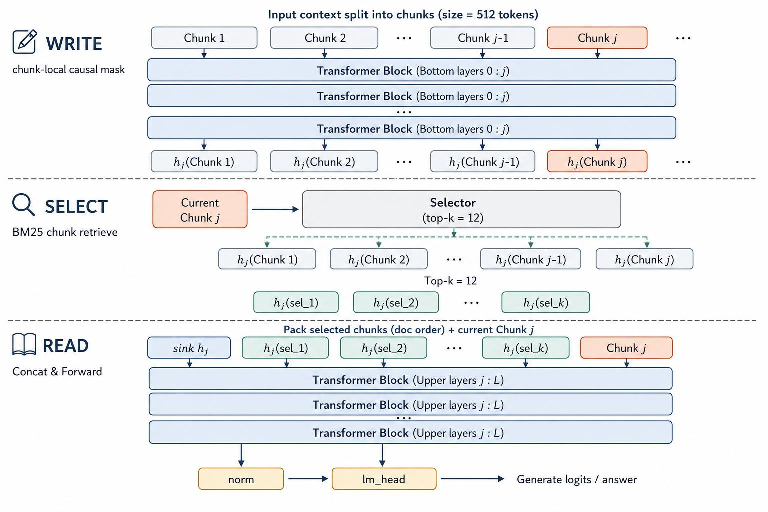
\includegraphics[width=\textwidth]{figures/Structure.pdf}}
\caption{\textbf{CoMem treats transformer depth as a cross-query reuse axis.}
\textsc{Write} stores an intermediate residual for each chunk,
\textsc{Select} retrieves a fixed working set, and \textsc{Read} resumes the
upper layers with the query present. The matched $j{=}0$ path retrieves the
same raw-text chunks but recomputes every layer. A small left-overlap during
Write restores lower-layer document context without increasing persistent
storage or per-query Read work.}
\label{fig:teaser}
\end{figure*}

Long-context language models face two different costs. Processing a long prompt
increases time to first token, while retaining its layer-wise key--value (KV)
states increases accelerator memory~\citep{transformer,pagedattention}. Both
costs recur when a document, conversation, or codebase answers many queries.

Existing methods usually reduce the \emph{token} axis. Text retrieval selects a
small raw-text prompt and then recomputes the full network~\citep{rag,
xu2024retrievallong}; KV compression retains fewer full-depth states
~\citep{streamingllm,h2o,snapkv,pyramidkv,minicache}; and chunk-cache systems
reuse request states when their contextual dependencies permit it
~\citep{cachecraft}. These approaches provide valuable operating points, but
they do not jointly offer independently writable cross-query memory objects,
bounded query-conditioned selection, and direct continuation from an
intermediate model depth.

We study that interface with \textbf{CoMem}. During \textsc{Write}, context
chunks run through layers $[0{:}j)$ and store their residuals. During
\textsc{Select}, a retriever chooses a fixed number of chunks. During
\textsc{Read}, their states are packed with the query and only layers
$[j{:}L)$ execute with full cross-chunk attention (Figure~\ref{fig:teaser}).
The split $j$ is a reuse knob: a deeper split prepays more work and stores the
same one-vector-per-token representation, but reduces per-query upper-layer
computation. The limiting case $j{=}0$ is a matched raw-text replay baseline
with the same retrieved chunks, order, sink, and mask.

This framing separates two effects that are easily conflated. \emph{Bounded
selection} removes most online tokens; \emph{depth reuse} skips lower-layer
recomputation on the selected tokens. The former produces the large
full-context speedups. The latter is smaller but measurable: with the same LoRA,
pack, and examples, $j{=}12$ gives a $1.403\times$ Read-phase speedup over
$j{=}0$ at a 3.12-point RULER cost. Its one-time Write becomes worthwhile only
under reuse---about 9 repeated queries at 32k and 26--28 at 128k in the measured
serving cohort. At equal GPU-resident online latency, raw-text replay remains
stronger on our mixed diagnostic cohort, so CoMem should be read as a
quality--latency--storage frontier rather than an accuracy replacement for RAG.

\paragraph{What limits fidelity?}
An intermediate residual can be linearly informative without being natively
compatible with the remaining layers. A lightweight self-distillation LoRA
repairs much of this interface mismatch. On a paired multikey diagnostic,
controlled Write variants show that missing lower-layer document context is a
major source of the remaining deployable gap; position remapping alone does not
repair it. A document-contextual control matches full replay on that diagnostic,
and a deployable 32-token overlap improves
92.5 to 98.5 while adding only a small theoretical increment to lower-layer
Write FLOPs. This result turns the fidelity analysis into an actionable design
principle: context belongs primarily on the Write side.

\paragraph{Contributions.}
\begin{itemize}[leftmargin=1.2em,itemsep=2pt]
\item \textbf{A cross-query intermediate-residual memory interface} combining
independent writes, bounded selection, and direct upper-layer continuation. Its
depth split makes computation reuse explicit rather than hiding it inside a
token-cache policy.
\item \textbf{A matched accounting of the frontier.} We separate bounded
selection from depth-only reuse, report persistent bytes, one-time Write,
per-query Read, external-store costs, and measured repeated-query crossover
points.
\item \textbf{A controlled interface diagnosis and repair.} Same-pack replay,
same-depth adaptation, a continuous-state oracle, and a context/position
factorization identify lower-layer Write context as a major source of error on
the paired multikey diagnostic; a small overlap-Write recovers most of that
observed gap without enlarging the store or Read working set.
\end{itemize}
